\documentclass{article}
\usepackage[utf8]{inputenc}
\usepackage{amsmath}

\usepackage{graphicx}
\usepackage{geometry}
\usepackage{xcolor}
\usepackage{tikz}
\usepackage{pifont}

\usepackage{utp-doc}

\begin{document}
	
	%
	% --- Título de la Lectura ---
	\practicatitle{AD.04.01.01: Lectura de Ciclos Termodinámicos}
	
	% --- Metadatos de la Actividad ---
	\textbf{Asignatura:} Termodinámica Automotriz \\
	\textbf{Unidad IV:} - Sistemas y Ciclos de Potencia de Gas
	
	\vspace{5mm}
	\hrule
	\vspace{5mm}

\section*{Introducción a los ciclos termodinámicos}

Los \hl{ciclos termodinámicos} son secuencias de \hl{procesos} que transforman \hl{energía térmica} en \hl{trabajo mecánico}, o viceversa. Son la base de funcionamiento de \hl{máquinas térmicas} como \hl{motores de combustión interna}, refrigeradores y bombas de calor. Comprender estos ciclos es fundamental para el \hl{análisis} y \hl{diseño} de \hl{sistemas energéticos} en la \hl{ingeniería automotriz}.

En esta lectura, exploraremos los \hl{ciclos ideales} de \hl{Carnot}, \hl{Otto} y \hl{Diesel}, que sirven como \hl{modelos teóricos} para entender los límites y el comportamiento de los motores reales.
\vspace{0.5cm}
\hrule
\vspace{0.5cm}

\section{El ciclo de Carnot: el límite ideal}

El \hl{ciclo de Carnot} es un \hl{ciclo termodinámico ideal} y \hl{reversible} que opera entre dos \hl{fuentes de calor} a \hl{temperaturas constantes}. Es de suma \hl{importancia teórica} porque establece el \hl{límite superior de eficiencia} para cualquier \hl{máquina térmica} que opere entre esas dos temperaturas. Aunque no es realizable en la práctica, sirve como \hl{referencia} para evaluar el \hl{rendimiento} de los ciclos reales.

El \hl{ciclo de Carnot} consta de cuatro \hl{procesos reversibles}:

\begin{itemize}
    \item \textbf{Expansión Isotérmica (1-2):} El \hl{fluido de trabajo} \hl{absorbe calor} ($Q_H$) de una \hl{fuente a alta temperatura} ($T_H$) mientras se \hl{expande}, realizando \hl{trabajo}.
    \begin{itemize}
        \item Ecuación del calor absorbido:
        $$
        	Q_H = T_H \Delta S_{12}
        $$
    \end{itemize}

    \item \textbf{Expansión Adiabática (2-3):} El fluido se expande \hl{sin intercambio de calor}, \hl{disminuyendo su temperatura} de $T_H$ a $T_L$ mientras realiza \hl{trabajo}.
    \begin{itemize}
        \item Ecuación de la relación de temperaturas y volúmenes:
        $$
        	T_2 V_2^{\gamma-1} = T_3 V_3^{\gamma-1}
        $$
    \end{itemize}

    \item \textbf{Compresión Isotérmica (3-4):} El fluido \hl{cede calor} ($Q_L$) a un \hl{sumidero a baja temperatura} ($T_L$) mientras se \hl{comprime}, requiriendo \hl{trabajo}.
    \begin{itemize}
        \item Ecuación del calor cedido:
        $$
        	Q_L = T_L \Delta S_{34}
        $$
    \end{itemize}

    \item \textbf{Compresión Adiabática (4-1):} El fluido se comprime \hl{sin intercambio de calor}, \hl{aumentando su temperatura} de $T_L$ a $T_H$ mientras se le \hl{aplica trabajo}.
    \begin{itemize}
        \item Ecuación de la relación de temperaturas y volúmenes:
        $$
        	T_4 V_4^{\gamma-1} = T_1 V_1^{\gamma-1}
        $$
    \end{itemize}
\end{itemize}

La \hl{eficiencia térmica} del \hl{ciclo de Carnot} ($\eta_{Carnot}$) se define como:

$$
	\eta_{Carnot} = 1 - \frac{T_L}{T_H}
$$

Donde $T_L$ es la \hl{temperatura absoluta} del \hl{sumidero de calor} y $T_H$ es la \hl{temperatura absoluta} de la \hl{fuente de calor}.

\begin{figure}[h!]
    \centering
    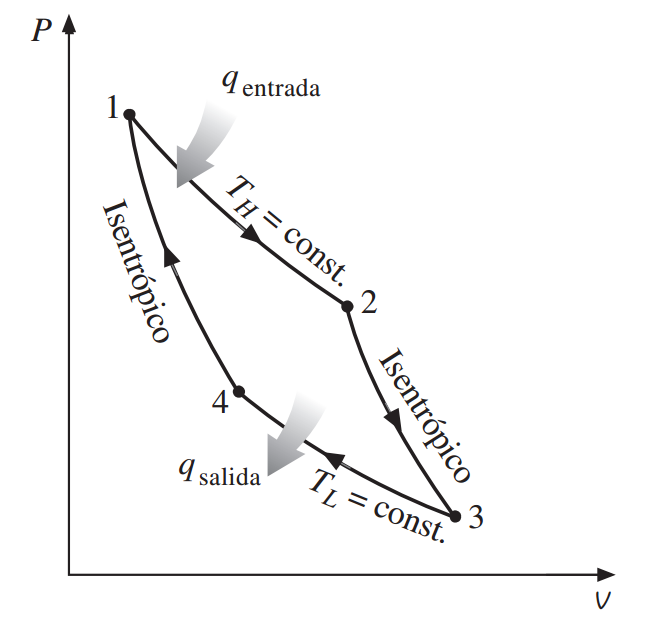
\includegraphics[width=0.45\textwidth]{diagrama-PV-carnot.png}
    \hfill
    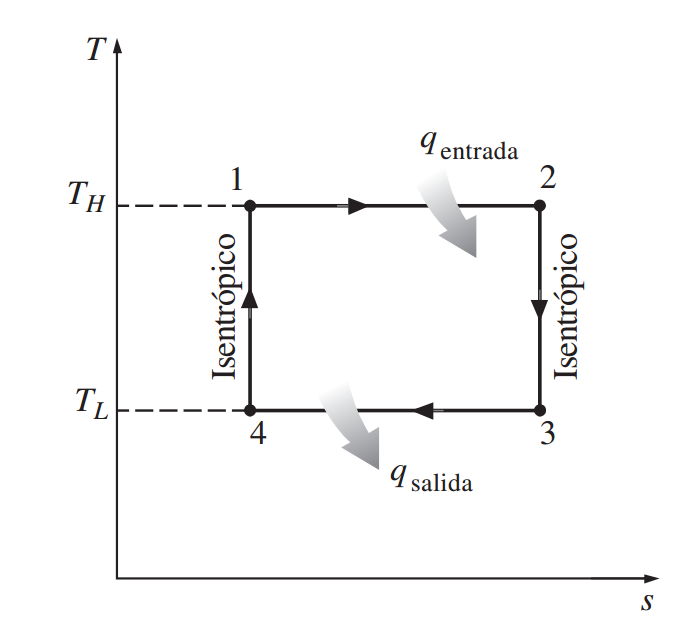
\includegraphics[width=0.45\textwidth]{diagrama-TS-carnot.png}
    \caption{Diagramas P-V (izquierda) y T-S (derecha) del ciclo de Carnot. {\small Fuente: Çengel, Y. A., Boles, M. A. (2011). Termodinámica.}}
    \label{fig:carnot_diagrams}
\end{figure}

\hrule

\section{El ciclo de Otto: motores de gasolina}

El \hl{ciclo de Otto} es el \hl{modelo ideal} para los \hl{motores de encendido por chispa} (\hl{motores de gasolina}). Se compone de cuatro \hl{procesos internamente reversibles}, dos \hl{adiabáticos} y dos \hl{isocóricos} (\hl{volumen constante}).

\begin{itemize}
    \item \textbf{Compresión Adiabática (1-2):} El \hl{aire-combustible} se \hl{comprime sin intercambio de calor}, \hl{aumentando su temperatura y presión}.
    \begin{itemize}
        \item \textbf{Relación de compresión} ($r$):
        $$
        	r = \frac{V_1}{V_2}
        $$
        
    \end{itemize}

    \item \textbf{Adición de Calor a Volumen Constante (2-3):} Se simula la \hl{combustión}, donde se \hl{añade calor} ($Q_{in}$) al sistema a \hl{volumen constante}, \hl{elevando drásticamente la presión y temperatura}.
    \begin{itemize}
        \item \textbf{Calor añadido}:
        $$
        	Q_{in} = m c_v (T_3 - T_2)
        $$
    \end{itemize}

    \item \textbf{Expansión Adiabática (3-4):} Los \hl{gases calientes} se \hl{expanden}, realizando \hl{trabajo} sobre el \hl{pistón} y \hl{disminuyendo su temperatura y presión}.

    \item \textbf{Rechazo de Calor a Volumen Constante (4-1):} Se simula la \hl{expulsión de gases de escape}, donde se \hl{cede calor} ($Q_{out}$) al ambiente a \hl{volumen constante}, \hl{disminuyendo la presión}.
    \begin{itemize}
        \item \textbf{Calor rechazado}:
        $$
        	Q_{out} = m c_v (T_4 - T_1)
        $$
    \end{itemize}
\end{itemize}

La \hl{eficiencia térmica} del \hl{ciclo de Otto} ($\eta_{Otto}$) se expresa como:

$$
	\eta_{Otto} = 1 - \frac{1}{r^{\gamma-1}}
$$

Donde $r$ es la \hl{relación de compresión} y $\gamma$ es la \hl{relación de calores específicos} ($c_p/c_v$).

\begin{figure}[h!]
    \centering
    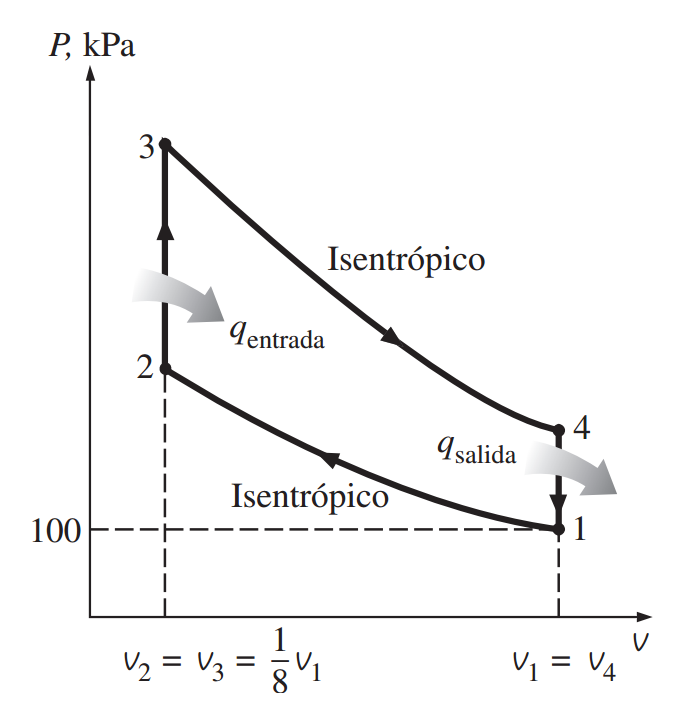
\includegraphics[width=0.45\textwidth]{diagrama-PV-Otto.png}
    \hfill
    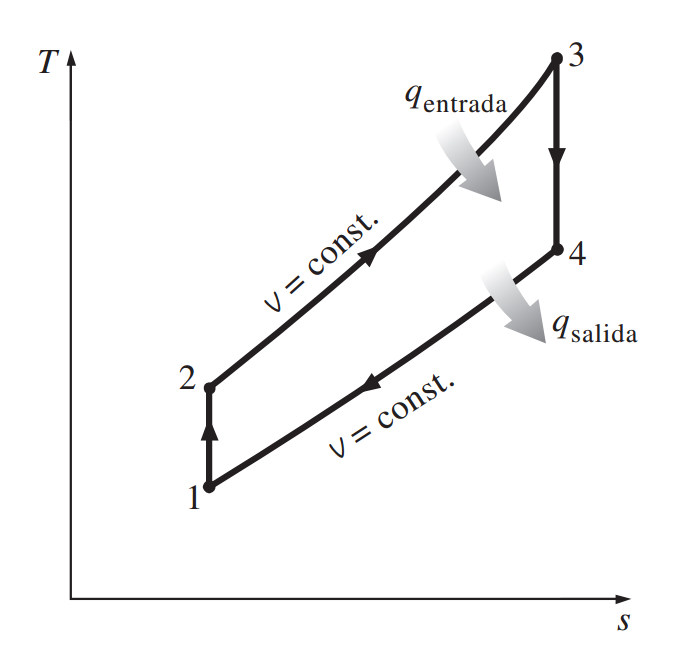
\includegraphics[width=0.45\textwidth]{diagrama-TS-Otto.png}
    \caption{Diagramas P-V (izquierda) y T-S (derecha) del ciclo de Otto. Fuente: Çengel, Y. A., \& Boles, M. A. (2011). *Termodinámica*.}
    \label{fig:otto_diagrams}
\end{figure}


\hrule

\section{El ciclo Diesel: motores de encendido por compresión}

El \hl{ciclo Diesel} es el \hl{modelo ideal} para los \hl{motores de encendido por compresión} (\hl{motores diésel}). A diferencia del \hl{ciclo de Otto}, la \hl{adición de calor} ocurre a \hl{presión constante}.

\begin{itemize}
    \item \textbf{Compresión Adiabática (1-2):} El \hl{aire} se \hl{comprime sin intercambio de calor}, \hl{aumentando su temperatura y presión}.

    \item \textbf{Adición de Calor a Presión Constante (2-3):} Se simula la \hl{combustión}, donde se \hl{añade calor} ($Q_{in}$) al sistema a \hl{presión constante}, \hl{elevando el volumen y la temperatura}.
    \begin{itemize}
        \item \textbf{Calor añadido}:
        $$
        	Q_{in} = m c_p (T_3 - T_2)
        $$
    \end{itemize}

    \item \textbf{Expansión Adiabática (3-4):} Los \hl{gases calientes} se \hl{expanden}, realizando \hl{trabajo} sobre el \hl{pistón} y \hl{disminuyendo su temperatura y presión}.

    \item \textbf{Rechazo de Calor a Volumen Constante (4-1):} Se simula la \hl{expulsión de gases de escape}, donde se \hl{cede calor} ($Q_{out}$) al ambiente a \hl{volumen constante}, \hl{disminuyendo la presión}.
    \begin{itemize}
        \item \textbf{Calor rechazado}:
        $$
           Q_{out} = m c_v (T_4 - T_1)
       $$
    \end{itemize}
\end{itemize}

La \hl{eficiencia térmica} del \hl{ciclo Diesel} ($\eta_{Diesel}$) se calcula con la siguiente fórmula:

$$
\eta_{Diesel} = 1 - \frac{1}{r^{\gamma-1}} \left[ \frac{r_c^{\gamma} - 1}{\gamma (r_c - 1)} \right]
$$

Donde $r$ es la \hl{relación de compresión} y $r_c$ es la \hl{relación de corte} (relación de volúmenes al final y al inicio de la adición de calor a presión constante).

\begin{figure}[h!]
    \centering
    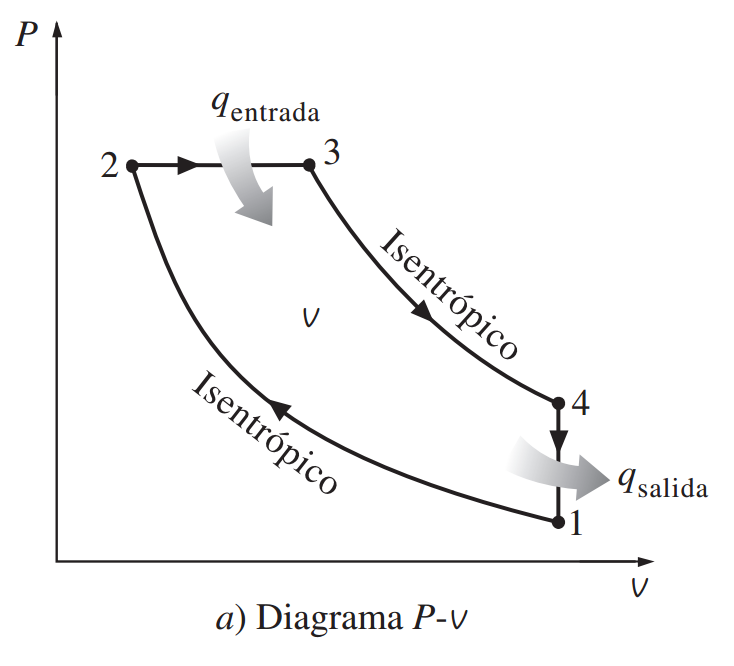
\includegraphics[width=0.45\textwidth]{Diagrama-PV-Diesel.png}
    \hfill
    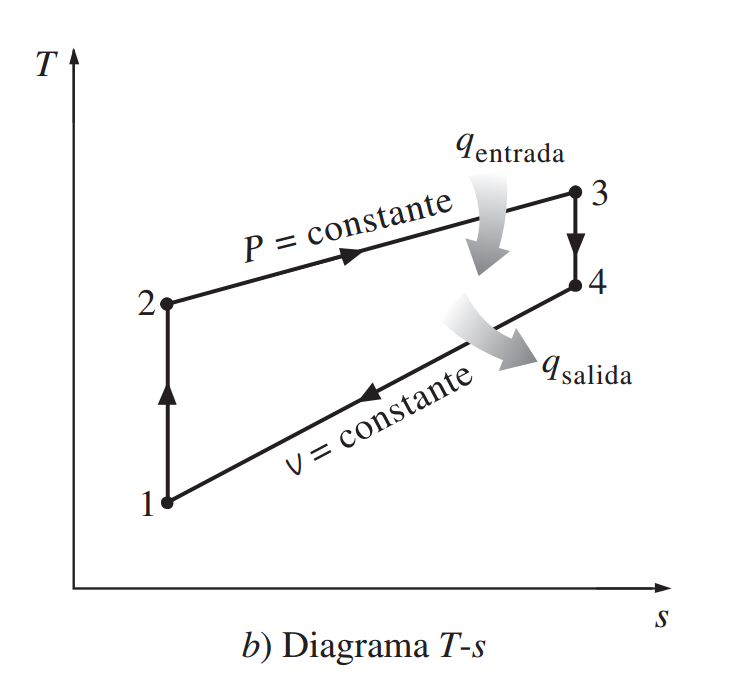
\includegraphics[width=0.45\textwidth]{diagrama-TS-Diesel.png}
    \caption{Diagramas P-V (izquierda) y T-S (derecha) del ciclo de Diesel. Fuente: Çengel, Y. A.,  Boles, M. A. (2011). Termodinámica.}
    \label{fig:diesel_diagrams}

\end{figure}

\hrule

\section{Comparación de ciclos y parámetros clave en motores}

Aunque los \hl{ciclos de Otto y Diesel} son \hl{modos ideales}, su \hl{comparación} nos permite entender las \hl{diferencias fundamentales} en el \hl{diseño} y \hl{operación} de los \hl{motores de gasolina y diésel}.

\begin{table}[h!]
\centering
\begin{tabular}{|l|l|l|}
\hline
\textbf{Característica} & \textbf{Ciclo de Otto (Gasolina)} & \textbf{Ciclo Diesel (Diésel)} \\
\hline
\textbf{Combustión} & Por \hl{chispa} (bujía) & Por \hl{compresión} (autoignición) \\
\hline
\textbf{Adición de Calor} & A \hl{volumen constante} & A \hl{presión constante} \\
\hline
\textbf{Combustible} & \hl{Gasolina} & \hl{Diésel} \\
\hline
\textbf{Relación de Compresión} & Típicamente \hl{más baja} (8:1 a 12:1) & Típicamente \hl{más alta} (14:1 a 25:1) \\
\hline
\textbf{Eficiencia} & Depende fuertemente de la \hl{relación de compresión} & Depende de la \hl{relación de compresión} y de \hl{corte} \\
\hline
\end{tabular}
\end{table}

\textbf{Parámetros Clave en Motores de Combustión Interna:}

\begin{itemize}
    \item \textbf{Potencia} ($W$): \hl{Tasa} a la que se realiza \hl{trabajo}. En motores, se refiere a la \hl{potencia generada} por el motor.
    \begin{itemize}
        \item \textbf{Ecuación general de potencia}:
        $$
        W = \frac{\text{Trabajo}}{\text{Tiempo}}
        $$
    \end{itemize}
    \item \textbf{Cilindrada} ($V_d$): \hl{Volumen total desplazado} por todos los \hl{pistones} en un ciclo. Es un \hl{indicador del tamaño del motor}.
    \begin{itemize}
        \item \textbf{Ecuación de cilindrada unitaria}:
        $$
        V_d = \frac{\pi D^2}{4} L
        $$
        Donde $D$ es el \hl{diámetro del cilindro} y $L$ es la \hl{carrera del pistón}.
    \end{itemize}
    \item \textbf{Rendimiento} (\hl{Eficiencia}): \hl{Relación} entre el \hl{trabajo útil obtenido} y la \hl{energía suministrada}. Puede ser \hl{térmica}, \hl{mecánica} o \hl{volumétrica}.
\end{itemize}


\hrule

\section*{Conclusión}

Los \hl{ciclos de Carnot, Otto y Diesel} son \hl{pilares fundamentales} en la \hl{termodinámica aplicada} a la \hl{ingeniería automotriz}. Aunque son \hl{idealizaciones}, proporcionan las \hl{herramientas conceptuales y analíticas} para entender el \hl{funcionamiento}, las \hl{limitaciones} y las \hl{oportunidades de mejora} en los \hl{motores de combustión interna}. La \hl{comprensión} de sus \hl{procesos}, \hl{eficiencias} y los \hl{parámetros clave} asociados es \hl{esencial} para el \hl{análisis} y \hl{diseño} de \hl{sistemas energéticos eficientes y sostenibles}.

\hrule

\section*{Referencias Bibliográficas}

\begin{itemize}
    \item Çengel, Y. A., \& Boles, M. A. (2011). \textit{Termodinámica} (6a. ed.). McGraw-Hill.
    \item Moran, M. J., Shapiro, H. N., Boettner, D. D., \& Bailey, M. B. (2018). \textit{Fundamentals of Engineering Thermodynamics} (9th ed.). Wiley.
    \item Payri, F., \& Desantes, J. M. (Coords.). (2011). \textit{Motores de combustión interna alternativos}. Editorial de la UPV.
\end{itemize}

\end{document}